%%%%%%%%%%%%%%%%%%%%%%%%%%%%%%%%%%%%%%%%%%%%%%%%%%%%%%%%%%%
\subsection{Apply statistical model to data}
%%%%%%%%%%%%%%%%%%%%%%%%%%%%%%%%%%%%%%%%%%%%%%%%%%%%%%%%%%%
%
%
\begin{frame}[t, negative]
	\subsectionpage
\end{frame}
%
%
\begin{lhframe}[rhgraphic={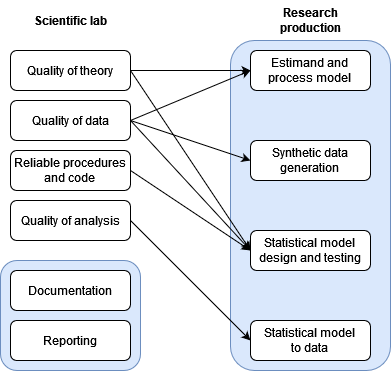
\includegraphics[scale=0.43]{lab_to_research.png}}]
	{What we have so far}
	
	\begin{enumerate}
		%
		\item measure: \\
		{\small replicated entropies $H^{O}_{ik}$ }
		%
		\item estimand: \\
		{\small $SI$ index, structural parameters, contrasts }
		%
		\item structural models: \\
		{\small total and direct effects }
		%
		\item probabilistic models: \\
		{\small three possible fitting models }
		%
		\item statistical models: \\
		{\small works as intended }
		%
		\item power: \\
		{\small enough }
		%
	\end{enumerate} 
	%
\end{lhframe}
%
%
\begin{lhframe}[rhgraphic={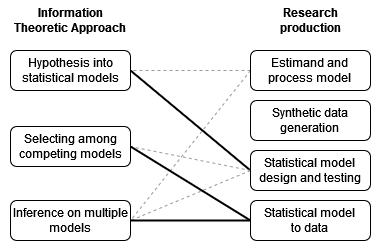
\includegraphics[scale=0.63]{ITA_to_research.png}}]
	{Information Theoretic Approach \cite{Anderson_2008, Chamberlain_1965} }
	
	The last step would be \textcolor{blue}{select the most fitting model} using the ITA,
	\begin{enumerate}
		%
		\item \sout{hypothesis into statistical models},
		\item select among competing models, 
		\item make inferences based on one or multiple models.
		%
	\end{enumerate}
	%
	the most fitting model based on information criteria,
	\begin{itemize}
		%
		\item WAIC \cite{Watanabe_2013}
		\item PSIS \cite{Vehtari_et_al_2021}
		%
	\end{itemize}
	%
\end{lhframe}
%
%
\begin{lhframe}[rhgraphic={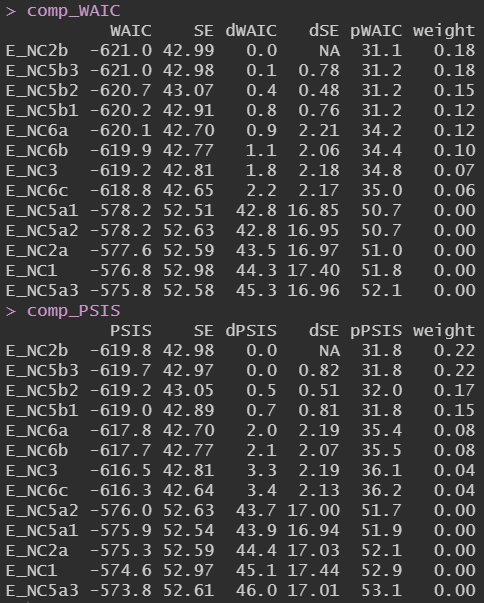
\includegraphics[scale=0.40]{models_table.png}}]
	{Competing models}
	%
	
	%
\end{lhframe}
%
%
